\documentclass[14pt]{beamer}
\usepackage[utf8]{inputenc}
\usepackage[T1]{fontenc}
\usepackage[frenchb]{babel}

\title{}
\date{\today}
\author{KI'018}

\usetheme{ki}

\begin{document}

\begin{frame}
    \titlepage
\end{frame}

% \sepframe{KI ? Ça se mange ?}

% \begin{frame}
%     \frametitle{Le KI}
%     KI = Club informatique de l'école
% \end{frame}

\sepframe{Vous nous connaissez pour ...}

\begin{frame}
    \frametitle{Le réseau des résidences}
    \begin{columns}
        \begin{column}{.6\textwidth}
            Géré à 100 \% par le KI
            \begin{itemize}
                \item Accueil des 1A
                \item Vente de routeurs et de câbles Ethernet
                \item Internet très haut débit
                \item Chasse aux DHCP pirates
            \end{itemize}
        \end{column}
        \begin{column}{.4\textwidth}
        % \vspace{0.5cm}
        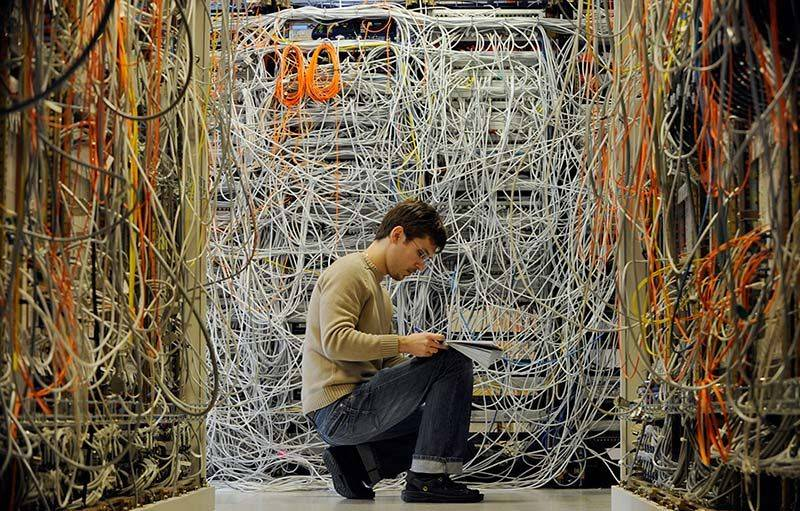
\includegraphics[width=\textwidth]{reseau.jpg}
        \end{column}
    \end{columns}
\end{frame}

\begin{frame}
    \frametitle{Dépannage}
    \begin{columns}
        \begin{column}{.6\textwidth}
            \begin{itemize}
                \item Assistance aux élèves
                \item Réparation d'ordinateurs
                \item Conseils et apprentissage
            \end{itemize}
        \end{column}
        \begin{column}{.4\textwidth}
        % \vspace{0.5cm}
        \includegraphics[width=\textwidth]{error.png}
        \end{column}
    \end{columns}
\end{frame}

\sepframe{Mais le KI c'est aussi ...}

\begin{frame}
    \frametitle{Les soirées jeux video}
    \begin{columns}
        \begin{column}{.5\textwidth}
        Une à deux fois par mois \\
        Snacks \& boissons \\
            \begin{itemize}
                \item Super Smash Bros
                \item Counter-Strike
                \item Battlefront II
                \item ???
            \end{itemize}
            % Une à deux fois par mois \\
            % \begin{itemize}
            %     \item Snacks \& boissons
            %     \item Découverte
            %     \item Détente
            % \end{itemize}
        \end{column}
        \begin{column}{.5\textwidth}
        % \vspace{0.5cm}
        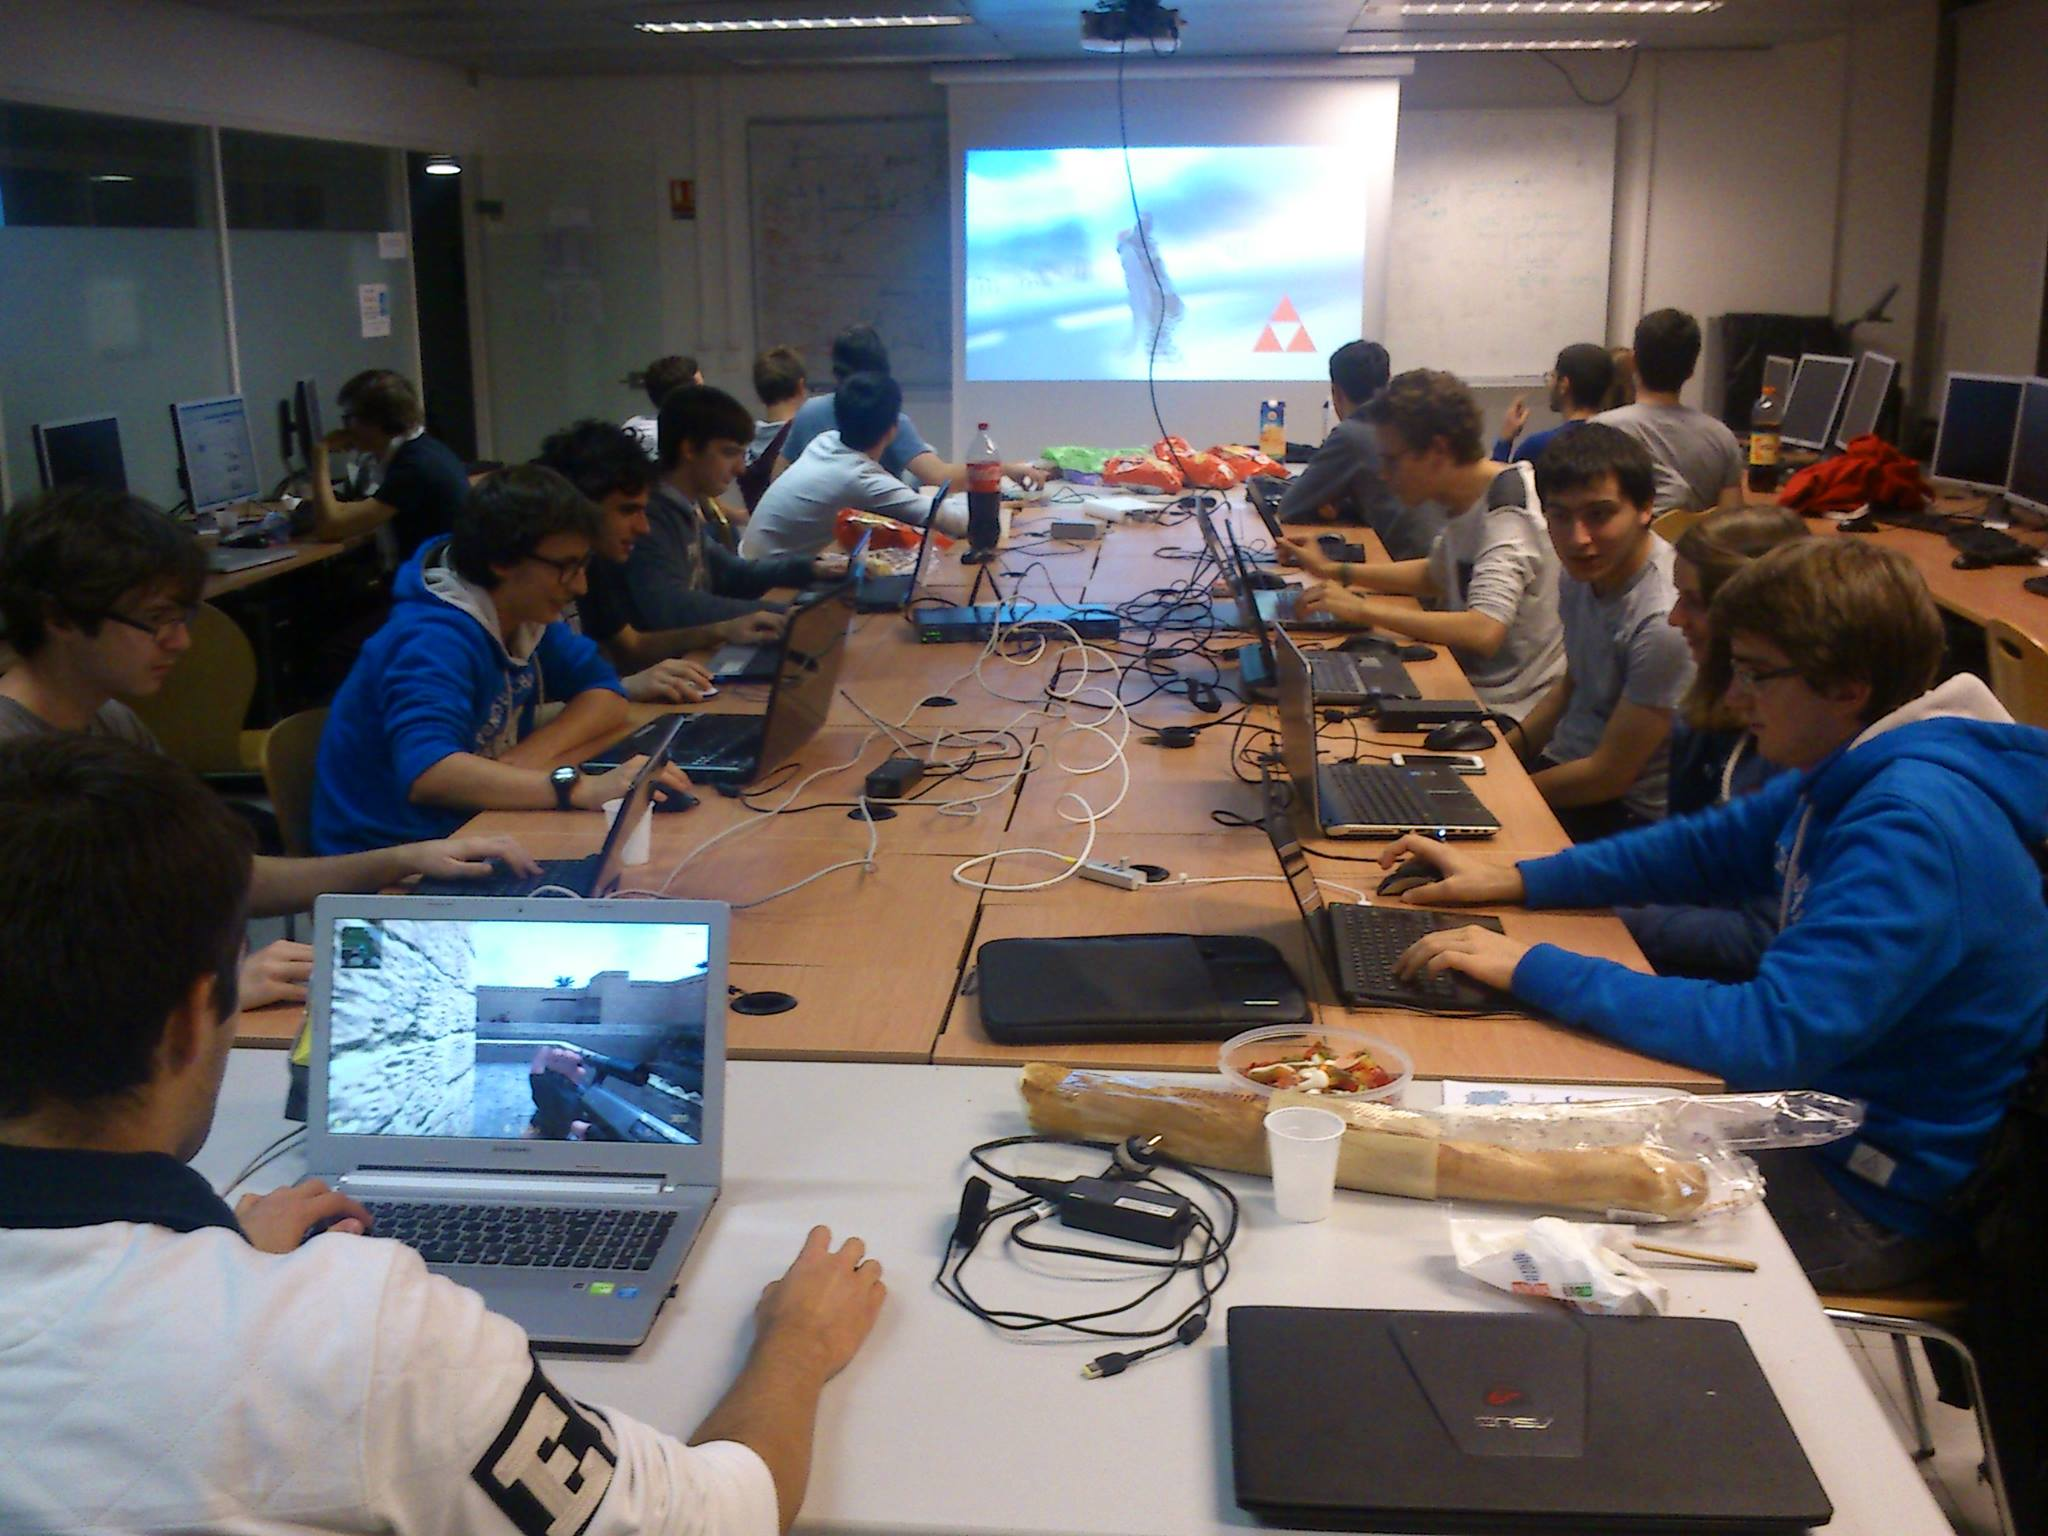
\includegraphics[width=\textwidth]{lan.jpg}
        \end{column}
  \end{columns}
\end{frame}

\begin{frame}
    \frametitle{Les formations}
    \begin{columns}
        \begin{column}{.3\textwidth}
        \begin{itemize}
            \item Linux
            \item \LaTeX
            \item Git
            \item Web
        \end{itemize}
        ~~~~(Pizzas)
        \end{column}
        \begin{column}{.7\textwidth}
        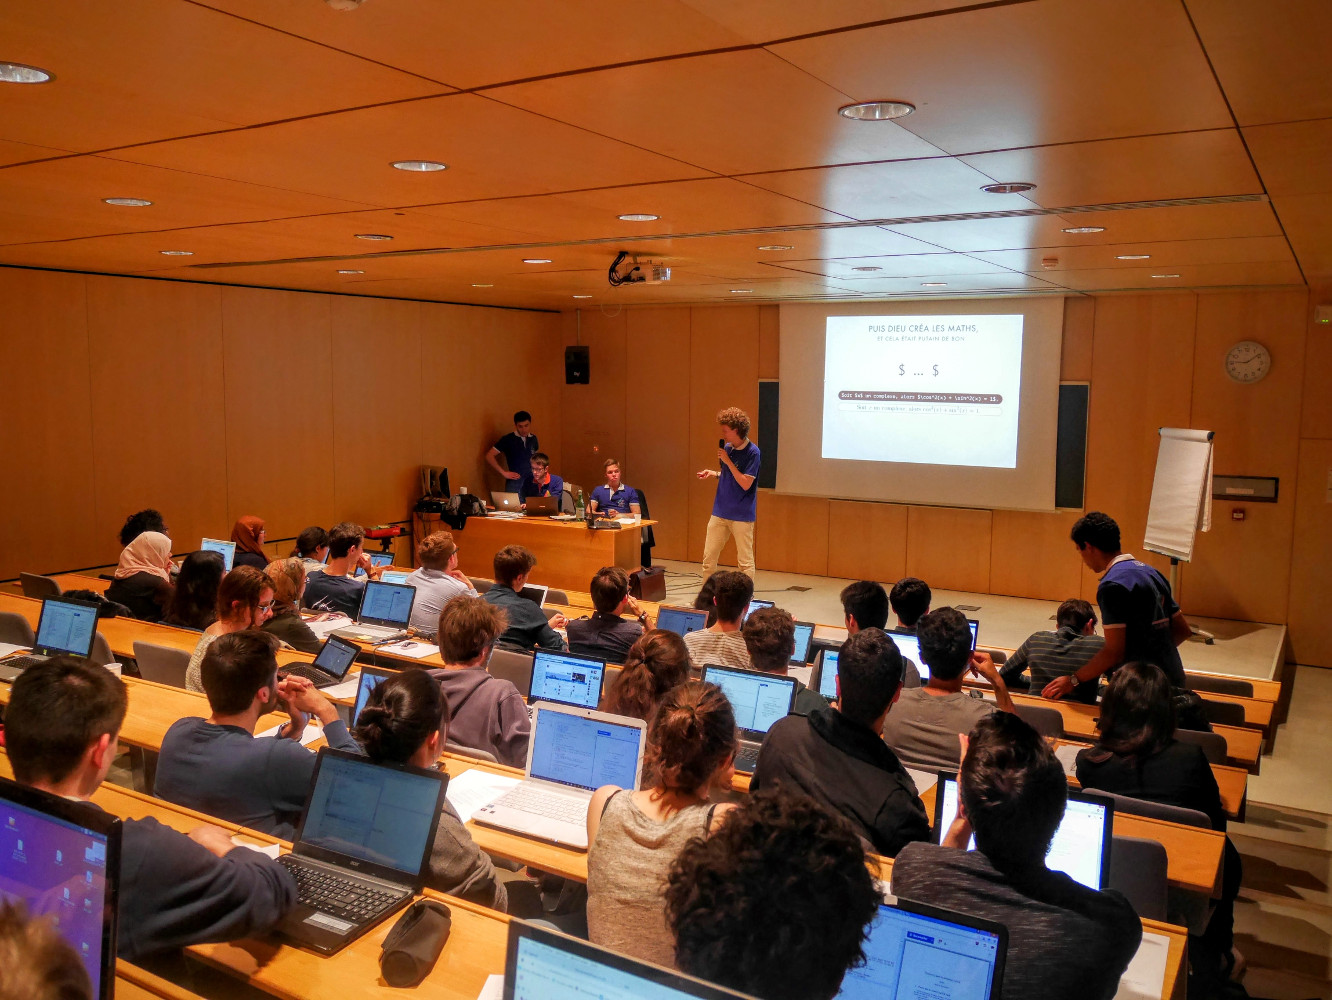
\includegraphics[width=\textwidth]{formations.jpg}
        \end{column}
  \end{columns}
\end{frame}

\begin{frame}
    \frametitle{Les centrales d'achat}
    \begin{columns}
        \begin{column}{.5\textwidth}
        Achats subventionnés par le KI
        \begin{itemize}
            \item Disques durs
            \item Clés USB KI
            \item Propositions ?
        \end{itemize}
        \end{column}
        \begin{column}{.5\textwidth}
            
\includegraphics[width=\textwidth]{achats.jpg}
        \end{column}
  \end{columns}
\end{frame}

\begin{frame}
    \frametitle{Nous contacter}
    \begin{columns}
        \begin{column}{.55\textwidth}
        \begin{itemize}
            \item P401
            \item clubinfo@upont.enpc.fr
            \item Page Facebook du KI
            \item uPont
        \end{itemize}
        \end{column}
        \begin{column}{.45\textwidth}
        {%
            \setlength{\fboxsep}{0pt}%
            \setlength{\fboxrule}{0.3pt}%
            \fbox{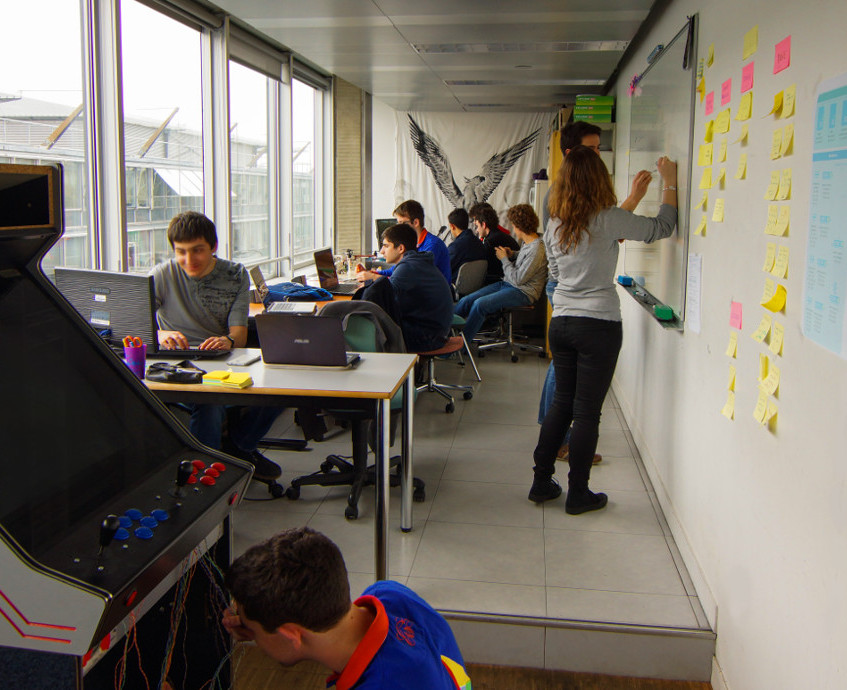
\includegraphics[width=\textwidth]{local2.jpg}}%
        }%
        \end{column}
  \end{columns}
\end{frame}

\begin{frame}
    \frametitle{uPont}
    \begin{center}
        
\includegraphics[height=0.6\textheight]{upont-1.png}
     \end{center}
\end{frame}

\end{document}
